\chapter{Stato dell'Arte}

In questo capitolo vengono presentati i fondamenti concettuali per il riconoscimento dei malware\
sulla base dei loro comportamenti.
Saranno introdotte le due principali tecniche di analisi, statica e dinamica, mettendone in evidenza\
punti di forza e limitazioni.
In seguito, l'attenzione verrà posta sull'analisi dinamica, approccio adottato in questa tesi,\
illustrandone i principi di machine learning adoperati per la sua realizzazione.

\section{Analisi Statica e Dinamica}

L'analisi statica si concentra sull'esame del codice del programma alla ricerca di specifiche sequenze di istruzioni,
denominate \textit{virus signature} (firma del virus)\mycite{christodorescu_jha_2003}.
L'efficacia dei sistemi basati su questa tecnica dipende dalla dimensione e dall'aggiornamento del database delle firme
e dall'impossibilità, per il software, di modificare nel tempo la propria struttura.
Per aggirare tali sistemi di rilevamento, i creatori di malware hanno sviluppato diverse tecniche di offuscamento,
che consentono di generare firme differenti rispetto a quelle originarie, rendendo più complessa la loro individuazione.
Tra le principali tecniche ritroviamo:

\begin{itemize}
    \item \textbf{Dead Code Insertion} (inserimento di codice morto): aggiunta di istruzioni prive di funzionalità
          ai fini malevoli, il cui unico scopo è alterare la firma rilevata\mycite{christodorescu_jha_2003}.
    \item \textbf{Code Transposition} (trasposizione del codice): riordinamento delle istruzioni,
          in modo che la rappresentazione binaria risulti differente pur mantenendo inalterata la logica di esecuzione\mycite{christodorescu_jha_2003}.
    \item \textbf{Register Reassignment} (riassegnazione dei registri): modifica dei registri utilizzati
          nelle operazioni interne al programma\mycite{christodorescu_jha_2003}.
    \item \textbf{Instruction Substitution} (sostituzione delle istruzioni): rimpiazzo di blocchi di codice
          con altri semanticamente equivalenti\mycite{christodorescu_jha_2003}.
\end{itemize}

Il continuo sviluppo di tecniche di offuscamento e l'aggiornamento dei database di firme ha dato vita a un vero e proprio ciclo vizioso,\
in cui l'evoluzione dei malware procede di pari passo con quella dei sistemi di rilevamento.\
Tale approccio, tuttavia, tende ad allontanarsi da ciò che realmente caratterizza un malware: i suoi comportamenti.

L'analisi dinamica rompe il ciclo generato dai limiti dell'approccio statico, poiché osserva i comportamenti\
effettivi del software durante l'esecuzione.\
In questo modo non solo riduce l'impatto delle tecniche di offuscamento sul codice,\
ma consente anche di evidenziare quei casi limite che l'analisi statica difficilmente riesce a cogliere,\
risultando complessivamente più efficace\mycite{Cesare2012-it}.
Per poter eseguire un analisi dinamica, esistono diverse tecniche:

\begin{itemize}
    \item \textbf{Hooking (Aggancio)}: intercetta chiamate API per monitorare o modificare il comportamento di un\
          programma. Utilizzato spesso dagli antivirus per controllare processi sospetti.\
          Limite: i malware possono rilevare la presenza di hook tramite checksum o controlli interni\mycite{Cesare2012-it}.\
          Un software per intercettare le chiamate API di Windows è \textit{Detours}\mycite{Detours}.

    \item \textbf{Dynamic Binary Instrumentation}(Strumentazione Dinamica del Binario): analizza e modifica\
          il codice binario mentre il programma è in esecuzione, permettendo di osservare ogni istruzione o comportamento\
          in tempo reale. Più difficile da rilevare rispetto all'hooking\mycite{Cesare2012-it}.\
          Un software che permette tale realizzazione è \textit{Dynamorio}\mycite{DynamoRIO_2025}.\

    \item \textbf{Virtualization}(Virtualizzazione): esegue un sistema operativo guest su hardware reale (host) isolato,\
          sfruttando meccanismi di separazione.\
          Veloce e relativamente sicuro, ma alcuni malware possono rilevare VM tramite differenze hardware/software\mycite{Cesare2012-it}.

    \item \textbf{Application Level Emulation}(Emulazione a Livello di Applicazione): crea un ambiente finto che emula\
          il sistema operativo e l'architettura di istruzioni per singole applicazioni.\
          Utile per analisi real-time e unpacking\footnote{Per \textit{unpacking} si intende il processo di estrazione del codice originario}, ma limitato nella fedeltà: i malware possono rilevare l'emulazione\
          usando istruzioni o API rare\mycite{Cesare2012-it}.

    \item \textbf{Whole System Emulation}(Emulazione dell'Intero Sistema): emula completamente l'hardware di un PC,
          permettendo l'installazione di un intero sistema operativo guest.\
          Molto utile per osservare comportamenti complessi, unpacking e analisi dettagliata, ma più lento rispetto alla virtualizzazione\mycite{Cesare2012-it}.
\end{itemize}

Un esempio concreto di implementazione della tecnica di \textbf{hooking} è presentato nell'articolo di \textit{Wtrace}\mycite{wtrace_net_2023},\
dove l'utilizzo della libreria \textit{Detours} permette di intercettare le chiamate API di un processo in esecuzione.\
Il risultato di tale analisi può essere osservato nella Figura~\ref{fig:api_call_example}, che mostra un output delle API Call registrate\
di un programma in esecuzione:\

\begin{figure}[htbp]
    \centering
    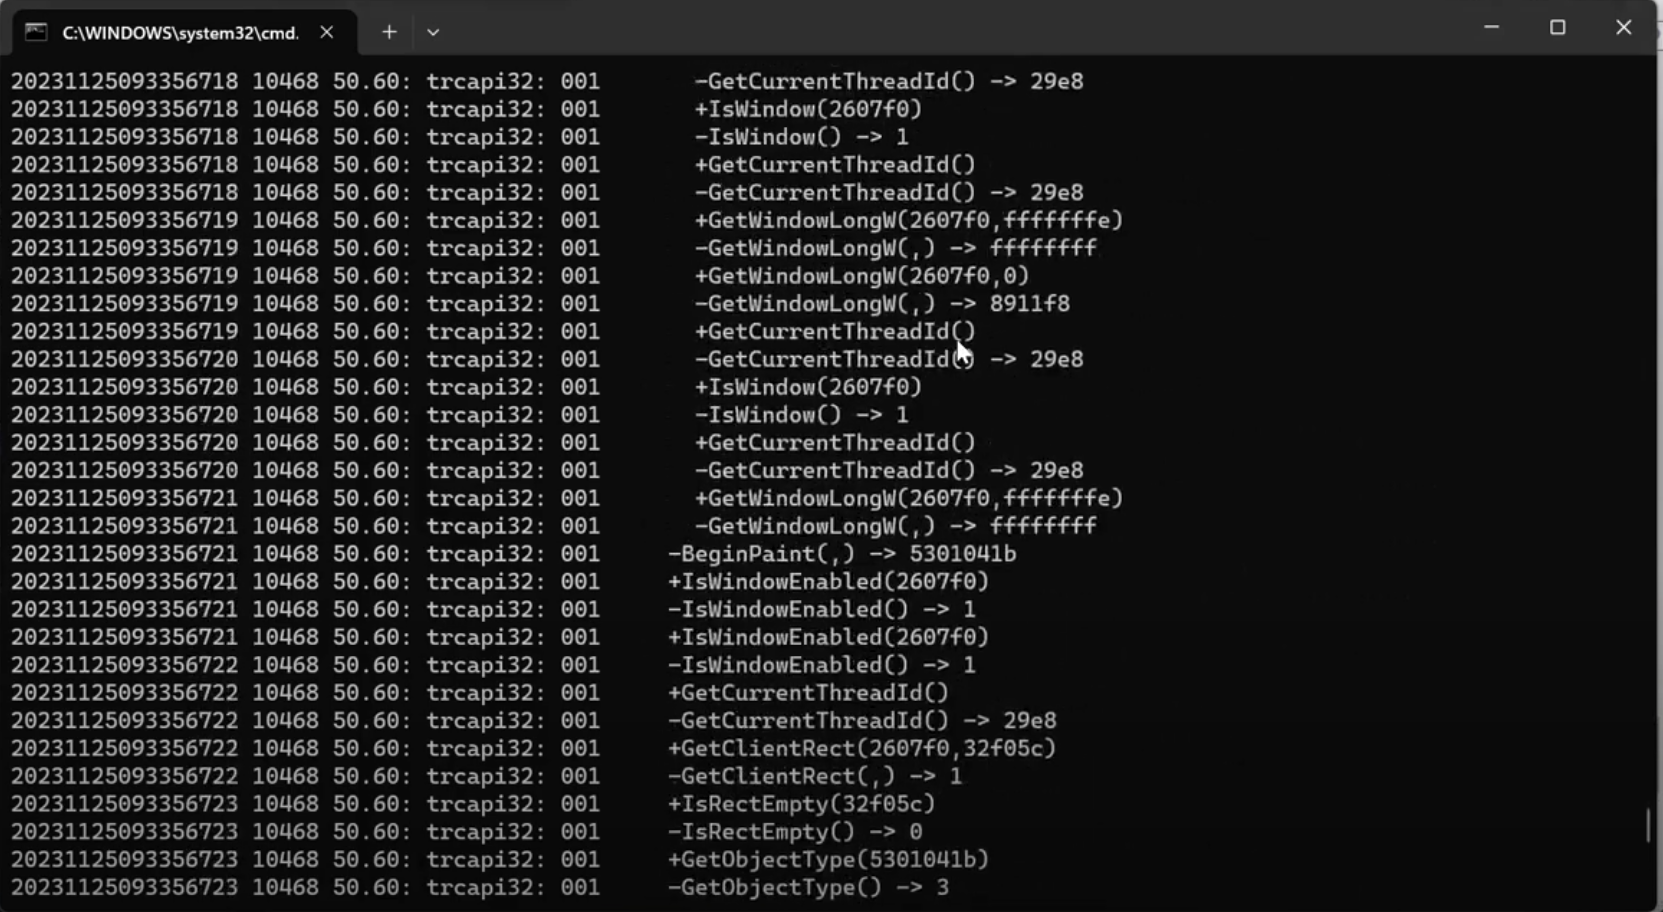
\includegraphics[width=1\textwidth]{./stato-dell-arte/imgs/api_call_example.png}
    \caption{API Call catturate}
    \label{fig:api_call_example}
\end{figure}

Tuttavia, il semplice elenco delle chiamate API non è sufficiente per mostrare la vera natura di un software.\
É necessario definire una logica di analisi che trasformi queste sequenze in informazioni discriminanti. In questa tesi\
tali logiche sono implementate tramite \textit{machine learning}.

\section{Machine Learning}

\subsection{Classificazione}

\subsection{Algoritmi di Classificazione}

\subsubsection{RandomForest}

\subsubsection{XGBoost}

\section{Metriche di valutazione}

\section{Approcci di Machine Learning per Windows PE Malware Detection}
